\section{Terrain Generation}

When users start CityCraft, they are first presented with an endless ocean and a menu panel, as shown in Figure \ref{fig:no_terr}.
This is the start of the generation process, and the ocean represents the blank canvas on which the rest of the world will be built.

\begin{figure}[H]
  \centering

  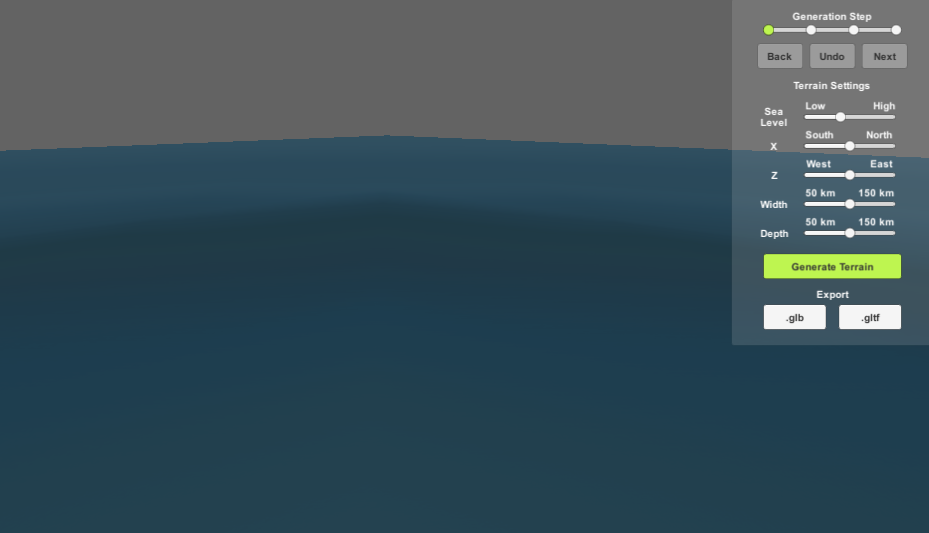
\includegraphics[width=0.7\textwidth]{figure/terrain_not_generated.png}
  \caption{The application state before the \textit{Generate Terrain} button has been pressed. The ocean is visible from the very beginning.}

  \label{fig:no_terr}
\end{figure}

The very first step of the generation processs is to generate the terrain, whose settings are adjusted in the top-right menu panel.
The terrain settings that the user can adjust are:
\begin{easylist}
  @ Sea level: modifies the water level.
  @ X/Z offset: offsets the sampling location along respective axis of the noise function, effectively changing the height values of the terrain.
  @ X/Z Size: adjusts the size of the entire terrain.
\end{easylist}

The terrain is generated by creating a surface mesh whose vertices are given height values sampled from a 4-layered Simplex noise function.
The terrain utilizes a single texture, which is repeated several times with randomized UV coordinates.
The terrain is also colored based on height values, forming snowy mountain tops and green valleys.
An example of a generated terrain is shown in Figure \ref{fig:terr}.

\begin{figure}[H]
  \centering

  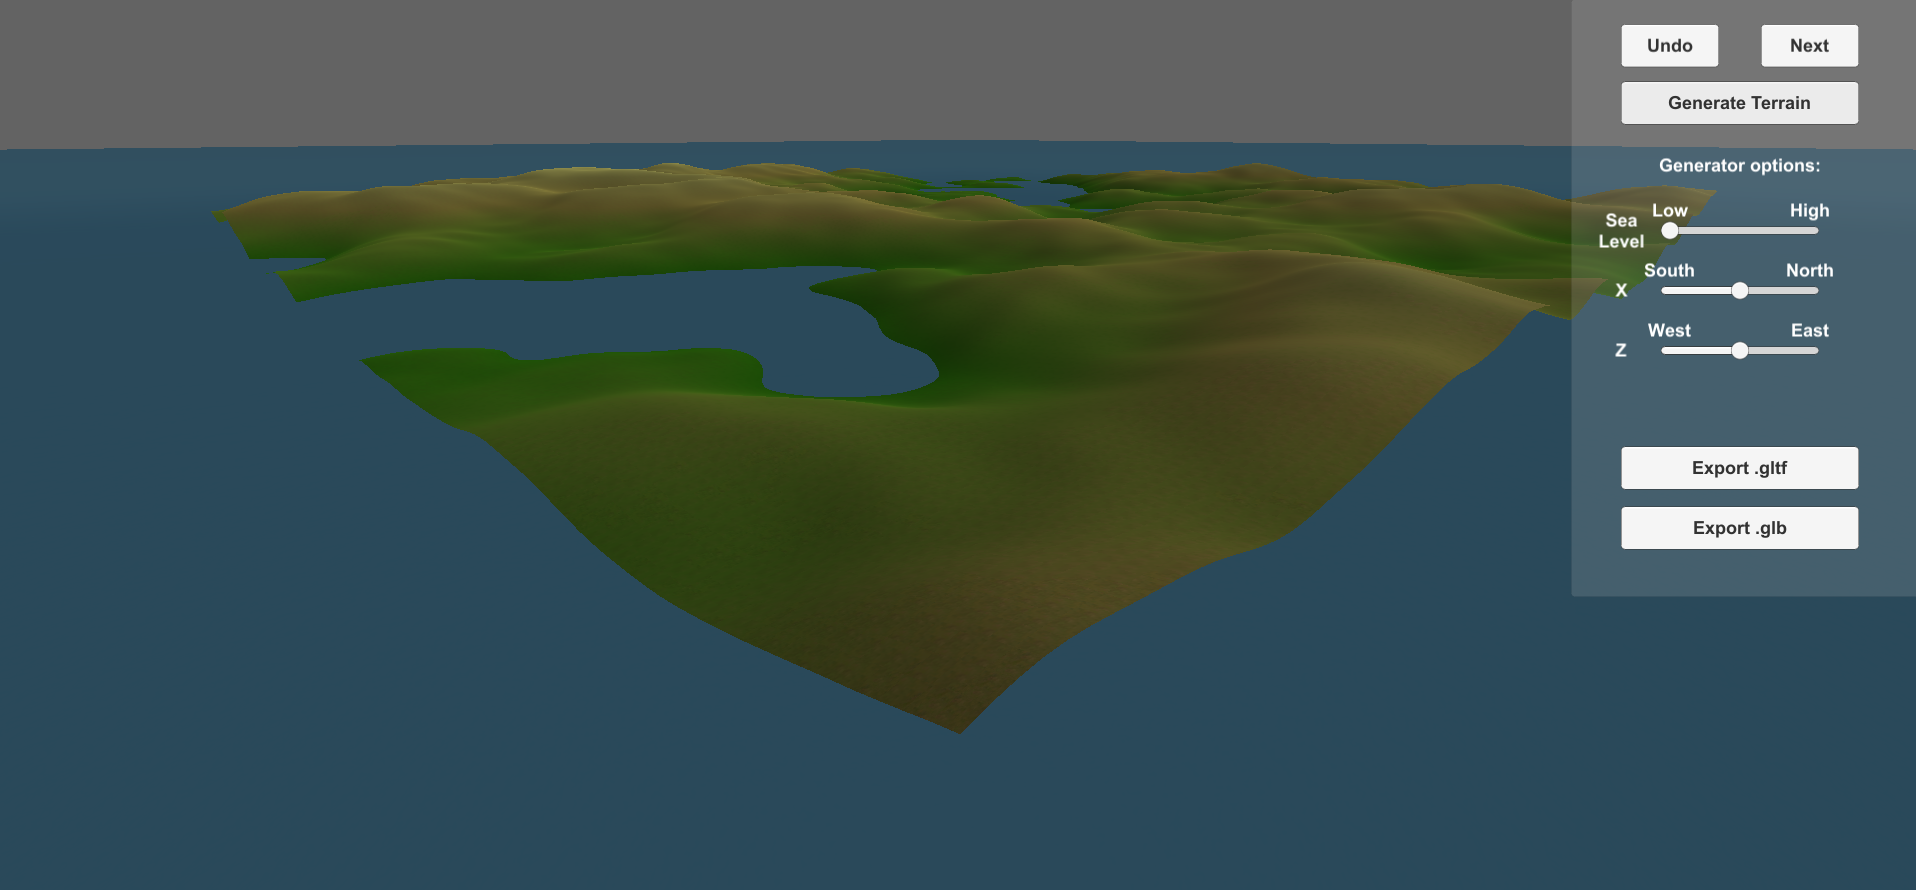
\includegraphics[width=0.7\textwidth]{figure/terrain_generated.png}
  \caption{The application state after \textit{Generate Terrain} has been pressed. The user may change settings and regenerate the terrain as many times as they like.}

  \label{fig:terr}
\end{figure}

The ocean was just implemented as a large textured plane that clips through the terrain, forming lakes at its intersections.

